\documentclass[border=3pt]{standalone}
% Preâmbulo compartilhado pelos diagramas TikZ da aula 14 (SLAM com EIF)
\usepackage[T1]{fontenc}
\usepackage[utf8]{inputenc}
\usepackage{lmodern}
\usepackage{amsmath}
\usepackage{xcolor}
\usepackage{tikz}
\usetikzlibrary{arrows.meta,angles,quotes,decorations.pathmorphing,decorations.pathreplacing,calc,
                positioning,shapes.geometric,shapes.misc,backgrounds,fit,
                math}

% Paleta (mesma dos SVGs originais)
\definecolor{dblue}{HTML}{2A5B8C}
\definecolor{dorange}{HTML}{B3541E}
\definecolor{dgreen}{HTML}{4A7C59}
\definecolor{dred}{HTML}{9C4B4B}
\definecolor{dcream}{HTML}{F4F1EA}
\definecolor{dshade}{HTML}{DDD7C9}

% Função gaussiana (não normalizada por padrão de escala visual)
\pgfmathdeclarefunction{gauss}{3}{%
  \pgfmathparse{1/(#3*sqrt(2*pi))*exp(-((#1-#2)^2)/(2*#3^2))}%
}

% Estilos comuns (prefixo d... para não colidir com chaves internas do pgf)
\tikzset{
  >={Stealth[length=2mm]},
  dguide/.style={gray!55, dashed, line width=0.4pt},
  daxis/.style={gray!60, line width=0.7pt, ->},
  dbody/.style={fill=black!3, draw=black!80, line width=1pt},
  dacc/.style={draw=dblue, line width=1pt},
  dlbl/.style={black!55, font=\small},
  dsub/.style={black!45, font=\footnotesize},
  dstate/.style={circle, draw=black!80, fill=dcream, line width=1pt,
                 minimum size=17mm, font=\large, inner sep=1pt},
  dobs/.style={circle, draw=black!80, fill=dshade, line width=1pt,
               minimum size=14mm, font=\large, inner sep=1pt},
  dbox/.style={rounded corners=2pt, draw=black!80, fill=dcream, line width=1pt,
               align=center, inner sep=6pt},
  dop/.style={circle, draw=black!80, fill=white, line width=1pt,
              minimum size=6mm, inner sep=0pt, font=\small},
  dtrans/.style={->, dblue, line width=1pt},
  dmeas/.style={->, dorange, line width=1pt},
  dcurve/.style={line width=1pt, dblue},
  dcurveb/.style={line width=1.4pt, dorange},
}

\begin{document}
\hyphenpenalty=10000 \exhyphenpenalty=10000 \tolerance=9999 \emergencystretch=3em
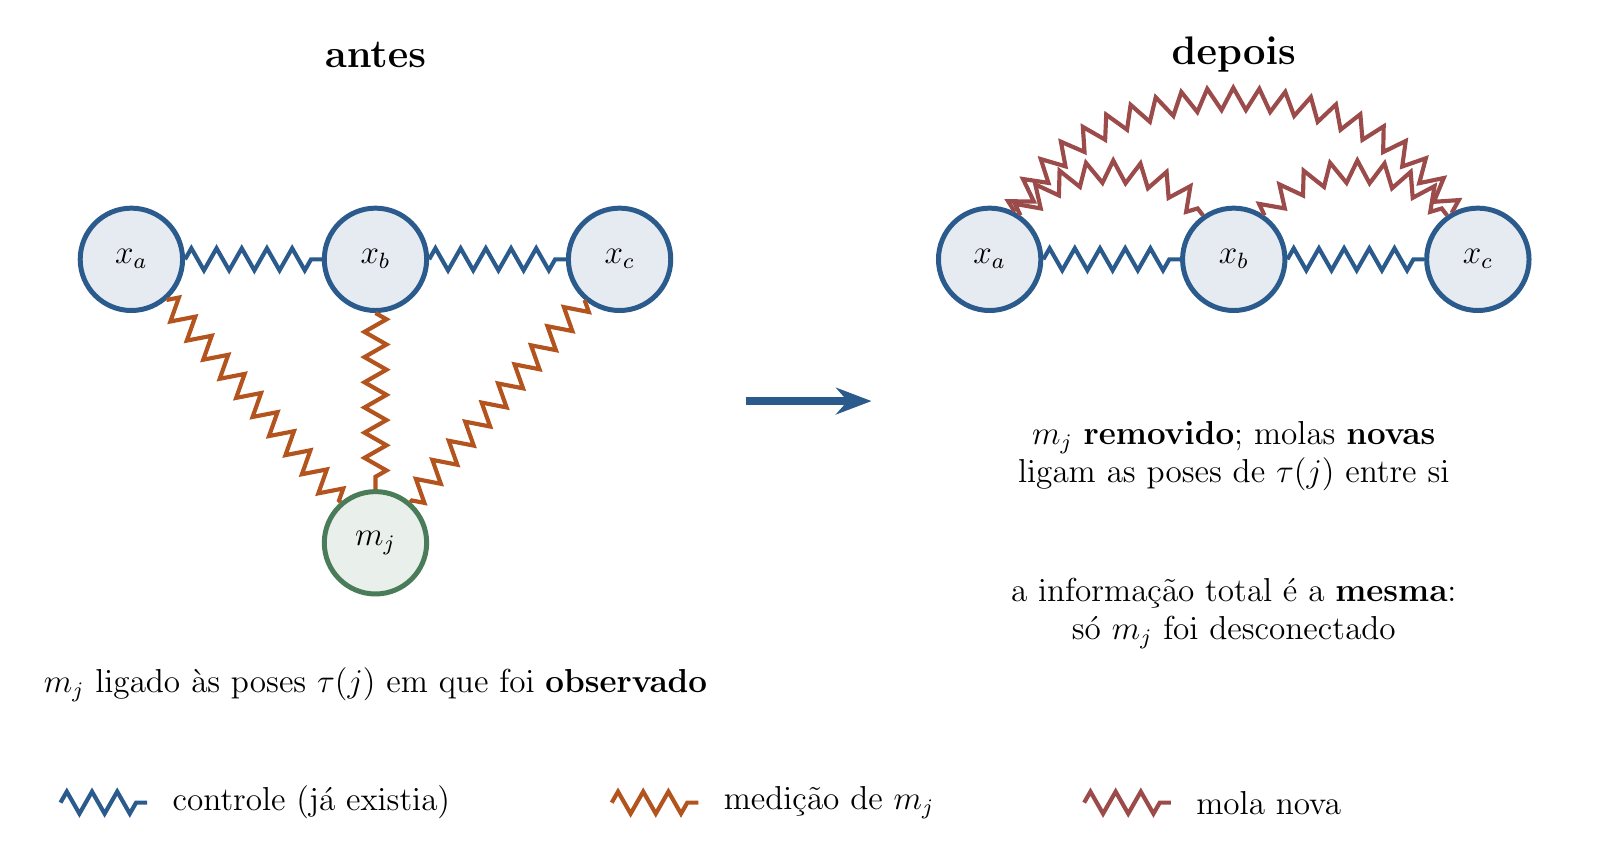
\begin{tikzpicture}[x=1cm,y=1cm]
\tikzset{p/.style={circle, draw=dblue, fill=dblue!12, line width=1.8pt, minimum size=1.3cm, font=\large},
        m/.style={circle, draw=dgreen, fill=dgreen!12, line width=1.8pt, minimum size=1.3cm, font=\large},
        sp/.style={decorate, decoration={zigzag, segment length=3.2mm, amplitude=1.4mm}, line width=1.5pt}}
\node[font=\Large\bfseries] at (4.3,8.6) {antes};
\node[p] (a1) at (1.2,6.0) {$x_a$}; \node[p] (a2) at (4.3,6.0) {$x_b$}; \node[p] (a3) at (7.4,6.0) {$x_c$};
\draw[sp, draw=dblue] (a1) -- (a2); \draw[sp, draw=dblue] (a2) -- (a3);
\node[m] (am) at (4.3,2.4) {$m_j$};
\draw[sp, draw=dorange] (a1) -- (am); \draw[sp, draw=dorange] (a2) -- (am); \draw[sp, draw=dorange] (a3) -- (am);
\node[font=\large, text width=8.6cm, align=center] at (4.3,0.6) {$m_j$ ligado às poses $\tau(j)$ em que foi \textbf{observado}};
\draw[dtrans, line width=3pt, -{Stealth[length=4.5mm]}] (9.0,4.2) -- (10.6,4.2);
\node[font=\Large\bfseries] at (15.2,8.6) {depois};
\node[p] (b1) at (12.1,6.0) {$x_a$}; \node[p] (b2) at (15.2,6.0) {$x_b$}; \node[p] (b3) at (18.3,6.0) {$x_c$};
\draw[sp, draw=dblue] (b1) -- (b2); \draw[sp, draw=dblue] (b2) -- (b3);
\draw[sp, draw=dred] (b1) to[bend left=55] (b2); \draw[sp, draw=dred] (b2) to[bend left=55] (b3); \draw[sp, draw=dred] (b1) to[bend left=62] (b3);
\node[font=\large, text width=8.6cm, align=center] at (15.2,3.5) {$m_j$ \textbf{removido}; molas \textbf{novas} ligam as poses de $\tau(j)$ entre si};
\node[font=\large, text width=8.6cm, align=center] at (15.2,1.5) {a informação total é a \textbf{mesma}: só $m_j$ foi desconectado};
\draw[sp, draw=dblue] (0.3,-0.9) -- (1.4,-0.9); \node[font=\large, anchor=west] at (1.6,-0.9) {controle (já existia)};
\draw[sp, draw=dorange] (7.3,-0.9) -- (8.4,-0.9); \node[font=\large, anchor=west] at (8.6,-0.9) {medição de $m_j$};
\draw[sp, draw=dred] (13.3,-0.9) -- (14.4,-0.9); \node[font=\large, anchor=west] at (14.6,-0.9) {mola nova};
\end{tikzpicture}
\end{document}
